% =====================================================================
% Póster A0 vertical — Optimización evolutiva de conjuntos de datos
% Esqueleto (fase 1): reparto de espacio, textos de borrador con cifras
% reales y huecos para las figuras. Compilar con:  latexmk -pdf poster.tex
% Poner \borradorfalse para ocultar los presupuestos de palabras.
% =====================================================================
\documentclass{article}
\usepackage[paperwidth=841mm,paperheight=1189mm,margin=0mm]{geometry}
\usepackage[T1]{fontenc}
\usepackage[utf8]{inputenc}
\usepackage{lmodern}  % matemáticas escalables a cualquier tamaño
\usepackage[scaled=1]{helvet}
\renewcommand{\familydefault}{\sfdefault}
\usepackage{amsmath}
\usepackage{array}
\usepackage{amssymb}
\usepackage{xcolor}
\usepackage{graphicx}
\usepackage{tikz}
\usepackage[most]{tcolorbox}
\usepackage{sansmath}  % matemáticas en la misma letra que el texto
\pagestyle{empty}
\setlength{\parindent}{0pt}

% ---------------------------------------------------------------------
% Modo borrador: muestra el presupuesto de palabras de cada bloque
% ---------------------------------------------------------------------
% Tema de color: 1 = blanco institucional (azul UC3M), 2 = gris carbón,
%                3 = minimalista (blanco, gris y naranja), 4 = verde azulado
\newcommand{\tema}{2}

\newif\ifborrador
\borradorfalse

% ---------------------------------------------------------------------
% Colores. Paleta fija por configuración (Okabe-Ito, apta para daltonismo):
% se usa igual en la leyenda de métodos y en todas las figuras.
% ---------------------------------------------------------------------
\definecolor{uctresm}{HTML}{000E78}    % estructura corporativo UC3M (medido en el logo)

\definecolor{tinta}{HTML}{1B1B1B}
\definecolor{cBase}{HTML}{4D4D4D}      % línea base (gris oscuro: referencia)
\definecolor{cA}{HTML}{CC79A7}         % A: solo selección (morado rosado)
\definecolor{cB}{HTML}{56B4E9}         % B: solo síntesis
\definecolor{cC}{HTML}{D55E00}         % C árboles: sistema propuesto
\definecolor{cGEP}{HTML}{009E73}       % C GEP


% ---------------------------------------------------------------------
% Temas: color principal, fondos suaves, barras de bloque y cabecera
% ---------------------------------------------------------------------
\definecolor{carbon}{HTML}{2F3542}
\definecolor{petroleo}{HTML}{0F5C63}
\definecolor{ambar}{HTML}{F2B33D}
\definecolor{ambarOsc}{HTML}{C98A12}  % ámbar oscuro: cifras sobre fondo blanco
\ifcase\tema\or
  % 1. Blanco institucional
  \colorlet{estructura}{uctresm}\definecolor{suave}{HTML}{DCE6F2}
  \colorlet{bloqueFondo}{estructura}\colorlet{bloqueTexto}{white}\colorlet{bloqueMarco}{estructura}
  \colorlet{cabFondo}{white}\colorlet{cabTitulo}{estructura}\colorlet{cabSub}{cC}\colorlet{cabTexto}{tinta}
  \colorlet{cabChip}{suave}\colorlet{cabChipTxt}{estructura}\colorlet{cabFilete}{estructura}
  \def\cabLogo{logos/logo_uc3m.png}\def\conFilete{1}
\or
  % 2. Gris carbón con acento ámbar
  \colorlet{estructura}{carbon}\definecolor{suave}{HTML}{E8E9ED}
  \colorlet{bloqueFondo}{estructura}\colorlet{bloqueTexto}{white}\colorlet{bloqueMarco}{estructura}
  \colorlet{cabFondo}{carbon}\colorlet{cabTitulo}{white}\colorlet{cabSub}{ambar}\colorlet{cabTexto}{white}
  \colorlet{cabChip}{white!12!carbon}\colorlet{cabChipTxt}{white}\colorlet{cabFilete}{ambar}
  \def\cabLogo{logos/logo_uc3m_blanco.png}\def\conFilete{1}
\or
  % 3. Minimalista: blanco, gris y un único acento naranja
  \colorlet{estructura}{tinta}\definecolor{suave}{HTML}{EEEEEE}
  \definecolor{bloqueFondo}{HTML}{EEEEEE}\colorlet{bloqueTexto}{tinta}\definecolor{bloqueMarco}{HTML}{CFCFCF}
  \colorlet{cabFondo}{white}\colorlet{cabTitulo}{tinta}\colorlet{cabSub}{cC}\colorlet{cabTexto}{tinta}
  \colorlet{cabChip}{suave}\colorlet{cabChipTxt}{cC}\colorlet{cabFilete}{cC}
  \def\cabLogo{logos/logo_uc3m.png}\def\conFilete{1}
\or
  % 4. Verde azulado (petróleo) con acento ámbar
  \colorlet{estructura}{petroleo}\definecolor{suave}{HTML}{DDEDEE}
  \colorlet{bloqueFondo}{estructura}\colorlet{bloqueTexto}{white}\colorlet{bloqueMarco}{estructura}
  \colorlet{cabFondo}{petroleo}\colorlet{cabTitulo}{white}\colorlet{cabSub}{ambar}\colorlet{cabTexto}{white}
  \colorlet{cabChip}{white!14!petroleo}\colorlet{cabChipTxt}{white}\colorlet{cabFilete}{ambar}
  \def\cabLogo{logos/logo_uc3m_blanco.png}\def\conFilete{1}
\fi

% ---------------------------------------------------------------------
% Tamaños de letra (a tamaño real A0, para leer a 1-2 m)
% ---------------------------------------------------------------------
\newcommand{\sizeTitle}{\fontsize{86}{96}\selectfont}
\newcommand{\sizeSub}{\fontsize{46}{56}\selectfont}
\newcommand{\sizeAuthor}{\fontsize{36}{44}\selectfont}
\newcommand{\sizeBlock}{\fontsize{54}{62}\selectfont}
\newcommand{\sizePanel}{\fontsize{38}{46}\selectfont}
\newcommand{\sizeBody}{\fontsize{28}{36}\selectfont}
\newcommand{\sizeSmall}{\fontsize{22}{28}\selectfont}
\newcommand{\sizeStat}{\fontsize{80}{88}\selectfont}
\newcommand{\sizeStatS}{\fontsize{60}{66}\selectfont}

\usetikzlibrary{arrows.meta, positioning, calc}
\newcommand{\menos}{\textendash}
\newcommand{\flecha}{\tikz[baseline=-0.25ex]\draw[-{Stealth[length=0.35em,width=0.35em]}, line width=0.09em] (0,0.3em) -- (1.1em,0.3em);}
\newcommand{\presupuesto}[1]{%
  \ifborrador\hfill{\sizeSmall\color{red!70!black}\textbf{[$\approx$#1 palabras]}}\fi}

% Hueco para una figura (se sustituye por \includegraphics en la fase 2)
\newcommand{\figura}[3]{% ancho, alto, descripción
  \begin{tikzpicture}
    \node[draw=gray!60, dashed, line width=2pt, fill=gray!8,
          minimum width=#1-3pt, minimum height=#2, inner sep=0pt,
          text width=0.85#1, align=center]
      {\sizeSmall\color{gray!45!black}\textbf{FIGURA}\\[4mm]#3};
  \end{tikzpicture}}

% Ficha de color con una cifra por configuración (panel 1)
\newcommand{\ficha}[3]{%
  \begin{tcolorbox}[enhanced, width=70mm, colback=#1!16, colframe=#1, boxrule=0pt, leftrule=4mm,
      arc=2mm, left=3mm, right=3mm, top=3mm, bottom=3mm, nobeforeafter, valign=center]
    {\sizeSmall\bfseries\color{#1!70!black}#2}\hfill{\sizeBody\bfseries #3}
  \end{tcolorbox}}

% Punto de color para la leyenda de configuraciones
\newcommand{\punto}[1]{\tikz[baseline=-0.8ex]\fill[#1] (0,0) circle (7mm);}

% Icono circular dibujado con TikZ (sin depender de fontawesome)
\newcommand{\icono}[1]{%
  \tikz[baseline=-1.2ex]{\fill[estructura] (0,0) circle (17mm);
    \node[text=white, font=\sizeBlock\bfseries] at (0,0) {#1};}}

% ---------------------------------------------------------------------
% Estilos de cajas
% ---------------------------------------------------------------------
% Bloque con barra de título de color (Introducción, Métodos, Resultados...)
\newtcolorbox{bloque}[2][]{enhanced, colback=white, colframe=bloqueMarco,
  boxrule=2.5pt, arc=6mm, left=12mm, right=12mm, top=10mm, bottom=10mm,
  title={#2}, fonttitle=\sizeBlock\bfseries, coltitle=bloqueTexto,
  colbacktitle=bloqueFondo, halign title=center, toptitle=6mm, bottomtitle=6mm,
  fontupper=\sizeBody\raggedright, #1}

% Panel numerado dentro de Resultados
\newtcolorbox{panel}[2][]{enhanced, colback=white, colframe=suave,
  boxrule=2pt, arc=4mm, left=9mm, right=9mm, top=7mm, bottom=7mm,
  fontupper=\sizeBody\raggedright,
  before upper={{\sizePanel\bfseries\color{estructura}#2\par}\vspace{6mm}}, #1}

% Sub-bloque de Métodos (título en el color principal, sin marco)
\newcolumntype{L}[1]{>{\raggedright\arraybackslash}m{#1}}
\newcommand{\subtitulo}[1]{{\sizePanel\bfseries\color{estructura}#1\par}\vspace{4mm}}

\begin{document}
\sansmath
\color{tinta}
% =====================================================================
% CABECERA
% =====================================================================
\noindent\begin{tcolorbox}[enhanced, sharp corners, boxrule=0pt,
  colback=cabFondo, width=\paperwidth, height=175mm, valign=center,
  left=25mm, right=25mm, top=0mm, bottom=0mm, nobeforeafter,
  % filete inferior de acento
  overlay={\ifnum\conFilete=1 \fill[cabFilete] (frame.south west) rectangle ([yshift=4mm]frame.south east);\fi}]
\begin{minipage}[c]{250mm}
  % Logo institucional a la izquierda
  \includegraphics[width=\linewidth]{\cabLogo}\par
  \vspace{8mm}
  % Cifras clave
  \begin{tcolorbox}[colback=cabChip, colframe=cabChip, boxrule=0pt,
      arc=4mm, left=4mm, right=4mm, top=4mm, bottom=4mm, width=121mm, nobeforeafter]\centering
    {\sizeStatS\bfseries\color{cabChipTxt}8\,\flecha\,7\par}\vspace{1mm}{\sizeSmall\color{cabChipTxt}columnas en California\par}
  \end{tcolorbox}\hfill
  \begin{tcolorbox}[colback=cabChip, colframe=cabChip, boxrule=0pt,
      arc=4mm, left=4mm, right=4mm, top=4mm, bottom=4mm, width=121mm, nobeforeafter]\centering
    {\sizeStatS\bfseries\color{cabChipTxt}\menos7,9\,\%\par}\vspace{1mm}{\sizeSmall\color{cabChipTxt}de error, mismo modelo\par}
  \end{tcolorbox}
\end{minipage}%
\hspace{25mm}%
\begin{minipage}[c]{515mm}\raggedright
  {\sizeTitle\bfseries\color{cabTitulo}Reducir dimensiones creando atributos, no solo eliminándolos\par}
  \vspace{6mm}
  {\sizeSub\color{cabSub}Programación genética multiárbol para regresión\par}
  \vspace{10mm}
  {\sizeAuthor\color{cabTexto}Mario Alberto Padilla Franco \quad·\quad Inteligencia Artificial Bioinspirada\par}
  \vspace{4mm}
  {\sizeSmall\color{cabTexto}\textbf{Palabras clave:} programación genética · construcción de atributos · reducción de dimensionalidad · regresión\par}
\end{minipage}
\end{tcolorbox}

\vspace{12mm}
% =====================================================================
% CUERPO: columna izquierda (introducción + métodos) y derecha (resultados)
% =====================================================================
\hspace*{20mm}%
\begin{minipage}[t]{255mm}\vspace{0pt}
% ------------------------- INTRODUCCIÓN -------------------------------
\begin{bloque}[height=182mm]{INTRODUCCIÓN}
  \presupuesto{70}\par
  \begin{tabular}{@{}m{38mm}@{\hspace{6mm}}L{180mm}@{}}
    \icono{?} & \textbf{\color{estructura}Problema:} ¿se puede transformar la matriz de atributos para que el mismo modelo cometa \emph{menos error} con \emph{menos columnas}?\\[8mm]
    \icono{!} & \textbf{\color{estructura}Idea:} evolucionar a la vez qué atributos originales se quedan y qué atributos nuevos se crean.\\[8mm]
    \icono{$\checkmark$} & \textbf{\color{estructura}Objetivo:} $e' < e$ con regresión lineal y $s < n$ columnas: síntesis \emph{y} reducción a la vez.
  \end{tabular}
\end{bloque}
\vspace{12mm}
% ------------------------- MÉTODOS -----------------------------------
\begin{bloque}[height=570mm]{MÉTODOS}
  \subtitulo{Cómo funciona}\presupuesto{20}\par
  \resizebox{\linewidth}{!}{%
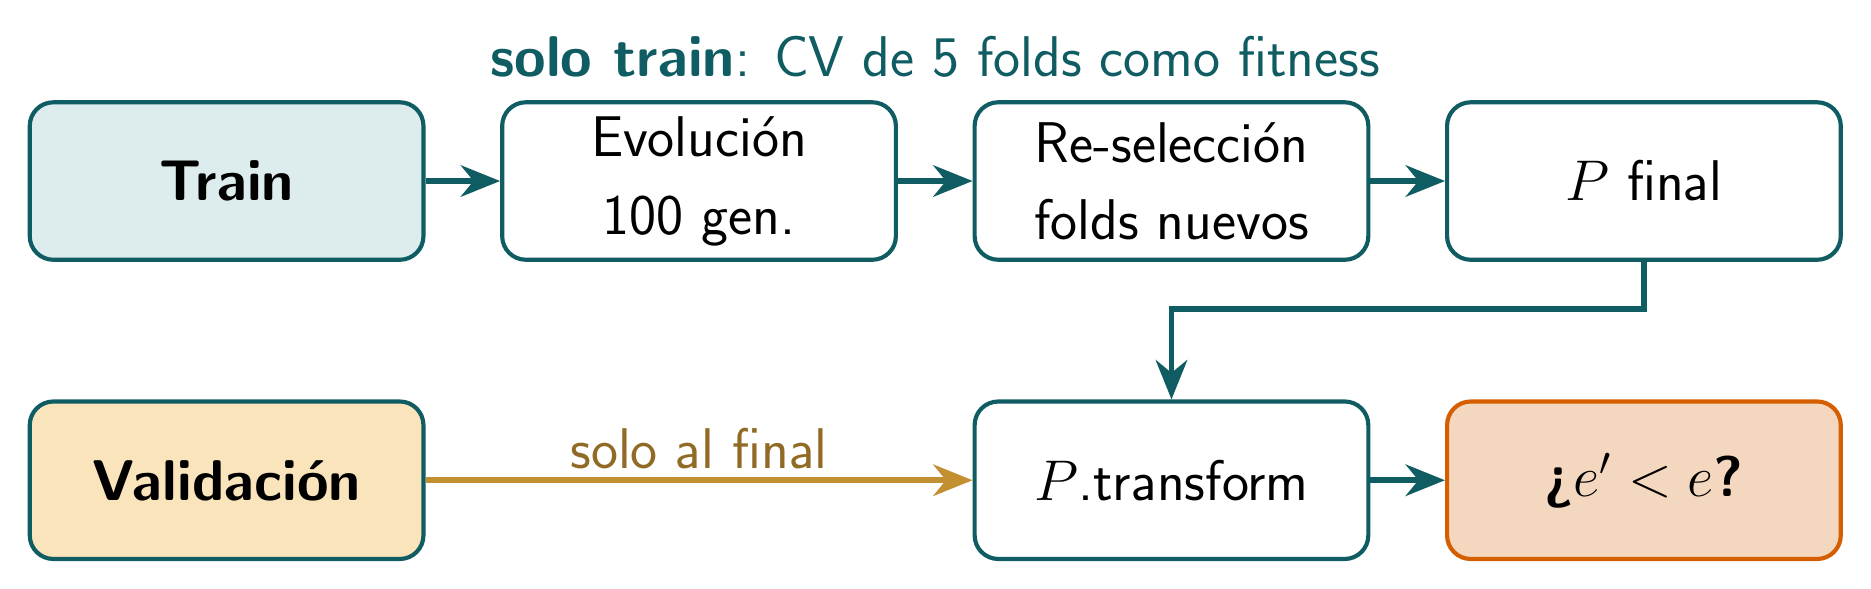
\begin{tikzpicture}[
    caja/.style={draw=estructura, line width=1.5pt, rounded corners=3mm, fill=white,
                 minimum width=50mm, minimum height=20mm, align=center, font=\sizeSmall},
    flecha/.style={-{Stealth[length=5mm,width=4mm]}, line width=2pt, color=estructura},
    x=1mm, y=1mm]
  % Fila superior: todo lo que aprende P sale de train
  \node[caja, fill=suave] (train) at (25,0) {\textbf{Train}};
  \node[caja] (evo) at (85,0) {Evolución\\100 gen.};
  \node[caja] (resel) at (145,0) {Re-selección\\folds nuevos};
  \node[caja] (pfin) at (205,0) {$P$ final};
  \draw[flecha] (train) -- (evo);
  \draw[flecha] (evo) -- (resel);
  \draw[flecha] (resel) -- (pfin);
  \node[font=\sizeSmall, color=estructura, anchor=south] at (115,12) {\textbf{solo train}: CV de 5 folds como fitness};
  % Fila inferior: validación se usa una vez, al final
  \node[caja, fill=ambar!35] (val) at (25,-38) {\textbf{Validación}};
  \node[caja] (trans) at (145,-38) {$P$.transform};
  \node[caja, fill=cC!25, draw=cC] (cmp) at (205,-38) {\textbf{¿$e' < e$?}};
  \draw[flecha, color=ambar!80!black] (val) -- node[above, font=\sizeSmall, color=ambar!60!black]{solo al final} (trans);
  \draw[flecha] (pfin.south) -- ++(0,-6) -| (trans.north);
  \draw[flecha] (trans) -- (cmp);
\end{tikzpicture}}\par
  \vspace{10mm}
  \subtitulo{El individuo}\presupuesto{45}\par
  \resizebox{\linewidth}{!}{%
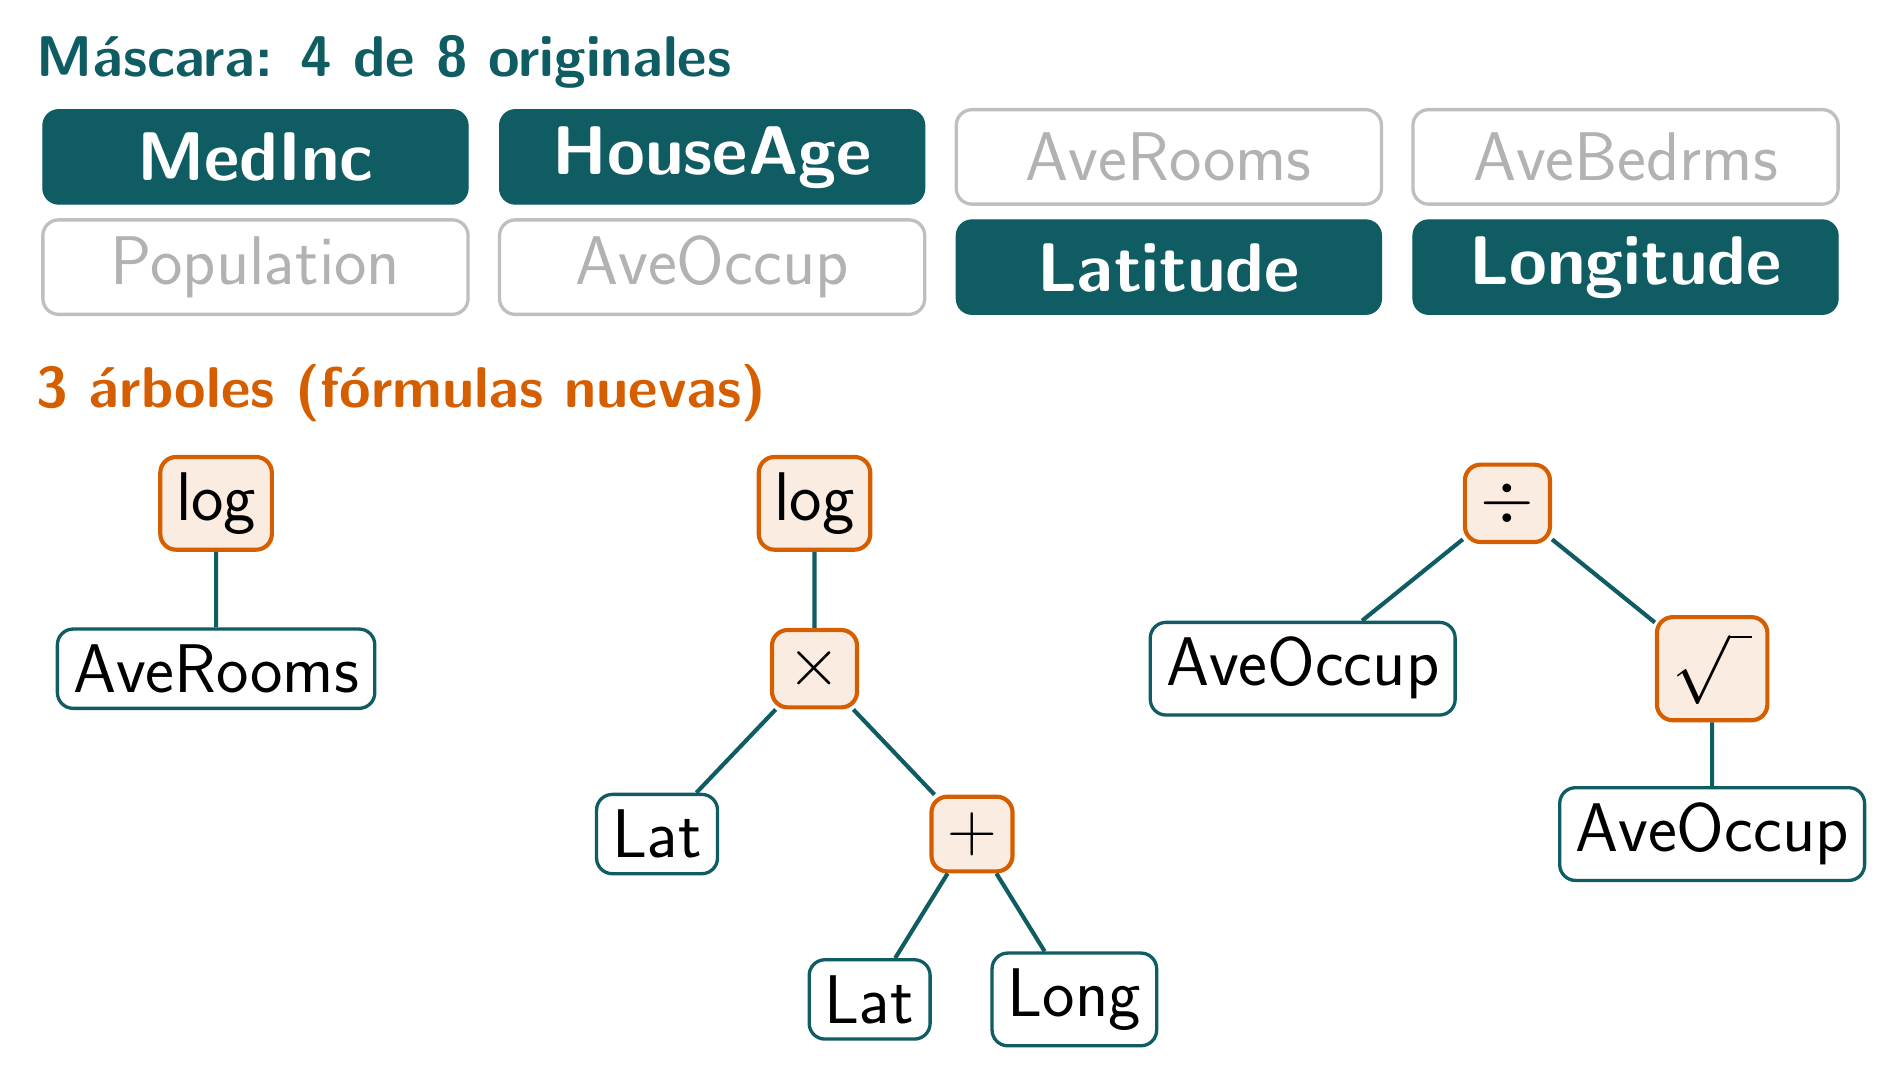
\begin{tikzpicture}[x=1mm, y=1mm,
    on/.style={draw=estructura, fill=estructura, text=white, rounded corners=2mm, minimum height=12mm,
               minimum width=54mm, font=\fontsize{25}{29}\selectfont\bfseries},
    off/.style={draw=gray!50, line width=1.2pt, fill=white, text=gray!60, rounded corners=2mm, minimum height=12mm,
               minimum width=54mm, font=\fontsize{25}{29}\selectfont},
    nodo/.style={draw=cC, line width=1.5pt, fill=cC!12, rounded corners=2mm, inner sep=2mm,
                 font=\fontsize{26}{30}\selectfont},
    hoja/.style={draw=estructura, line width=1.2pt, fill=white, rounded corners=2mm, inner sep=2mm,
                 font=\fontsize{26}{30}\selectfont},
    level distance=21mm, sibling distance=40mm, edge from parent/.style={draw=estructura, line width=1.5pt}]
  % Máscara de originales (8 bits, en dos filas)
  \node[anchor=west, font=\sizeSmall\bfseries, color=estructura] at (0,82) {Máscara: 4 de 8 originales};
  \foreach \nombre/\estado [count=\i] in {MedInc/on, HouseAge/on, AveRooms/off, AveBedrms/off}
    \node[\estado] at ({29+(\i-1)*58}, 70) {\nombre};
  \foreach \nombre/\estado [count=\i] in {Population/off, AveOccup/off, Latitude/on, Longitude/on}
    \node[\estado] at ({29+(\i-1)*58}, 56) {\nombre};
  % Tres árboles (interruptores activos)
  \node[anchor=west, font=\sizeSmall\bfseries, color=cC] at (0,40) {3 árboles (fórmulas nuevas)};
  \node[nodo] at (24,26) {log}
    child {node[hoja] {AveRooms}};
  \node[nodo] at (100,26) {log}
    child {node[nodo] {$\times$}
      child {node[hoja] {Lat}}
      child {node[nodo] {$+$} child[sibling distance=26mm] {node[hoja] {Lat}} child[sibling distance=26mm] {node[hoja] {Long}}}};
  \node[nodo] at (188,26) {$\div$}
    child[sibling distance=52mm] {node[hoja] {AveOccup}}
    child[sibling distance=52mm] {node[nodo] {$\sqrt{\ }$} child {node[hoja] {AveOccup}}};
\end{tikzpicture}}\par
  {\sizeSmall Ejemplo real (California, semilla 4): 7 columnas, $s<n=8$.\par}
  \vspace{4mm}
  \textbf{Fitness:} MAE en validación cruzada (5 folds) sobre train; si dos individuos difieren menos de $\varepsilon$, gana el más simple.\par
  \vspace{3mm}
  {\sizeSmall Población 100 · 100 generaciones · torneo 3 · elitismo 2 · 3 árboles de profundidad $\leq 3$ · parámetros elegidos con un piloto solo sobre train · funciones: $+$, $-$, $\times$, $\div$, $\sqrt{\ }$, $\log$ (protegidas)\par}
  \vspace{10mm}
  \subtitulo{Configuraciones}\presupuesto{45}\par
  \begin{tabular}{@{}c@{\hspace{5mm}}l@{}}
    \punto{cBase} & \textbf{Línea base:} todos los originales\\[2mm]
    \punto{cA}    & \textbf{A:} solo selección\\[2mm]
    \punto{cB}    & \textbf{B:} solo síntesis (sin límite)\\[2mm]
    \punto{cC}    & \textbf{C árboles:} sistema propuesto\\[2mm]
    \punto{cGEP}  & \textbf{C GEP:} misma idea con GEP
  \end{tabular}\par
  \vspace{3mm}
  \vspace{3mm}
  A y B quitan una de las dos piezas de C: comparándolas se ve qué aporta cada una (ablación).\par
  \vspace{4mm}
  {\sizeSmall California (20\,640 filas, $n=8$) y Diabetes (442 filas, $n=10$) · 30 semillas por configuración · hipótesis H1--H5 fijadas antes de ejecutar (veredicto en Conclusiones)\par}
\end{bloque}
\end{minipage}%
\hspace{15mm}%
\begin{minipage}[t]{531mm}\vspace{0pt}
% ------------------------- RESULTADOS --------------------------------
\begin{bloque}[height=764mm, left=8mm, right=8mm]{RESULTADOS}
  % Fila 1
  \begin{minipage}[t]{318mm}\vspace{0pt}
  \begin{panel}[height=310mm]{1. Crear atributos reduce el error en California}
    \includegraphics[width=\linewidth]{figuras/resultado_cajas.pdf}\par\vspace{3mm}
    C baja el MAE un 7,9\,\% (0,522 $\rightarrow$ 0,481) en el 97\,\% de las semillas ($p<10^{-5}$). Quitar atributos (A) no mejora; crearlos (B, C) sí. B logra la mejor mediana, pero empeora $e$ en 3 de 30 ejecuciones (C: 1).\presupuesto{45}\par
    \vspace{6mm}
    {\sizeSmall\bfseries Cambio mediano del MAE en California\par}\vspace{3mm}
    % Valores: results/analysis/estadistica.json (descriptive.california.*.rel_improvement_median)
    \ficha{cA}{A}{0,0\,\%}\hfill\ficha{cB}{B}{\menos9,4\,\%}\hfill\ficha{cC}{C}{\menos7,9\,\%}\hfill\ficha{cGEP}{C-GEP}{\menos8,3\,\%}
  \end{panel}
  \end{minipage}\hfill
  \begin{minipage}[t]{190mm}\vspace{0pt}
  \begin{panel}[height=310mm]{2. Menos columnas y menos error}
    \presupuesto{40}\par
    {\sizePanel\bfseries California\par}
    {\sizeStat\bfseries\color{ambarOsc}8\,\flecha\,7\hspace{3mm}{\sizePanel columnas}\par}
    \vspace{3mm}Error (MAE): \textbf{\menos7,9\,\%}\par\vspace{6mm}
    {\sizePanel\bfseries Diabetes\par}
    {\sizeStat\bfseries\color{ambarOsc}10\,\flecha\,8\hspace{3mm}{\sizePanel columnas}\par}
    \vspace{3mm}Error (MAE): \textbf{sin diferencia fiable}\par\vspace{6mm}
    \includegraphics[width=\linewidth]{figuras/originales_conservados.pdf}\par
    {\sizeSmall \% de las 30 ejecuciones de C (California).\par}
  \end{panel}
  \end{minipage}

  \vspace{10mm}
  % Fila 2
  \begin{minipage}[t]{254mm}\vspace{0pt}
  \begin{panel}[height=220mm]{3. Los atributos eliminados vuelven transformados}
    \presupuesto{60}\par
    \includegraphics[width=\linewidth]{figuras/transformaciones.pdf}\par\vspace{2mm}
    \textbf{Izq.:} distancia al número típico de habitaciones. \textbf{Der.:} raíz con signo que comprime los extremos. AveRooms y AveOccup están en las fórmulas del 80\,\% y el 87\,\% de las ejecuciones.\par\vspace{3mm}
    \textbf{Diabetes:} \emph{age} se conserva en el 0\,\% de las ejecuciones, pero aparece dentro de las fórmulas en el 70\,\% (p.\,ej. $\text{sex}\cdot\text{age}$).\par
  \end{panel}
  \end{minipage}\hfill
  \begin{minipage}[t]{254mm}\vspace{0pt}
  \begin{panel}[height=220mm]{4. En Diabetes, la mejora no se sostiene}
    \includegraphics[width=\linewidth]{figuras/diabetes_particiones.pdf}\par\vspace{3mm}
    Con la partición original y 30 semillas, \menos1,3\,\% ($p=0{,}005$), pero en 5 particiones nuevas C solo mejora en 1. {\sizeSmall Figura: mediana de 10 semillas por partición; negativo = menos error.}\presupuesto{40}
  \end{panel}
  \end{minipage}

  \vspace{10mm}
  % Fila 3
  \begin{minipage}[t]{254mm}\vspace{0pt}
  \begin{panel}[height=170mm]{5. Árboles y GEP: misma mediana, distinta fiabilidad}
    \centering\includegraphics[width=0.75\linewidth]{figuras/fiabilidad_mutacion.pdf}\par\raggedright\par\vspace{3mm}
    Mismo MAE típico ($p=0{,}14$), pero 11/30 ejecuciones con árboles fallan en la búsqueda. \textbf{Exploratorio:} más mutación ayuda (no significativo). {\sizeSmall *Tasa final.}\presupuesto{40}
  \end{panel}
  \end{minipage}\hfill
  \begin{minipage}[t]{254mm}\vspace{0pt}
  \begin{panel}[height=170mm]{Limitaciones}
    \presupuesto{55}\par
    · Falta comparar con transformaciones fijas hechas a mano (p.\,ej., $\log$).\\[2mm]
    · Validación pequeña en Diabetes (88 filas).\\[2mm]
    · Árboles frente a GEP mezcla representación e intensidad de mutación.\\[2mm]
    · C seguía mejorando en la generación 100.\\[2mm]
    · Ayuda a la regresión lineal, no a Random Forest.
  \end{panel}
  \end{minipage}
\end{bloque}
\end{minipage}

\vspace{12mm}
% =====================================================================
% CONCLUSIONES
% =====================================================================
\hspace*{20mm}%
\begin{bloque}[width=801mm, height=126mm, nobeforeafter, left=8mm, right=8mm]{CONCLUSIONES}
  \begin{tabular}{@{}*{5}{m{36mm}@{\hspace{5mm}}L{104mm}@{\hspace{6mm}}}@{}}
    \icono{1} & {\sizeSmall\bfseries\color{estructura}H1 · C mejora en California: apoyada}\newline Reduce columnas \emph{y} error a la vez. &
    \icono{2} & {\sizeSmall\bfseries\color{estructura}H3 · Crear frente a quitar: apoyada}\newline La mejora viene de crear atributos, no de quitarlos. &
    \icono{3} & {\sizeSmall\bfseries\color{estructura}H5 · Coste de $s<n$: apoyada}\newline Cuesta poco, y C falla menos que B. &
    \icono{4} & {\sizeSmall\bfseries\color{estructura}H2 · Diabetes: apoyada (nula)}\newline No hay mejora fiable (6 particiones). &
    \icono{5} & {\sizeSmall\bfseries\color{estructura}H4 · Árboles = GEP: apoyada, con matiz}\newline Mismo error; los árboles fallan más en la búsqueda.
  \end{tabular}
\end{bloque}

\vspace{12mm}
% =====================================================================
% PIE: referencias + QR
% =====================================================================
\hspace*{20mm}%
\begin{minipage}[c]{801mm}\sizeSmall\raggedright
  \textbf{\color{estructura}Referencias.}
  [1] Muñoz et al. (2019). M3GP para regresión simbólica. \emph{Memetic Computing} 11(2).
  [2] Tran, Xue y Zhang (2016). PG para construcción y selección de atributos. \emph{Memetic Computing} 8(1).
  [3] Virgolin, Alderliesten y Bosman (2020). Atributos compactos con PG. \emph{Swarm Evol. Comput.} 53.
  [4] Koza (1992). \emph{Genetic Programming}. MIT Press.
  [5] Ferreira (2001). Gene Expression Programming. \emph{Complex Systems} 13(2).
  [6] Efron et al. (2004). Least angle regression (Diabetes). \emph{Ann. Statist.} 32(2).
  [7] Pace y Barry (1997). Sparse spatial autoregressions (California). \emph{Stat. Probab. Lett.} 33(3).\par
\end{minipage}

\end{document}
